\chapter{Análise Bibliográfica sobre Uso de Inteligência Artificial para Detecção de Malware, por João Víctor Siqueira}

\section{Planejamento do estudo}
\label{StrawHat972:PlanEst}

Uma das maiores ameaças da cibersegurança nos dias de hoje é justamente o \textit{malware}, que se trata de um \textit{software} malicioso que foi desenvolvido intencionalmente para infiltrar e danificar o sistema computacional de um usuário sem o consentimento do mesmo. A fim de proteger o computador de uma possível infecção ou até mesmo ser capaz de remover um \textit{malware} de um sistema já comprometido, é essencial detectar um \textit{malware} com precisão, mas isso é uma tarefa difícil visto que nem sempre é trivial discernir se um determinado programa é ou não malicioso. 

Nesse contexto é que entra a ideia de pesquisar formas de realizar a detecção de \textit{malware} de forma mais precisa, e essa ideia casa perfeitamente com o uso de Inteligência Artificial, visto que um dos ramos dessa área da Ciência da Computação trata justamente de reconhecimento de padrões e classificação.

Dessa forma, o trabalho em questão busca compreender como é dado o uso das técnicas de Inteligência Artificial para detecção de \textit{softwares} maliciosos baseando-se em uma análise bibliográfica a qual será direcionada pelas seguintes questões:

\begin{itemize}
    \item Quais os principais conceitos relacionados a detecção de \textit{malware} com auxilio de IA?
    \item Como se deu a evolução das pesquisas acerca da detecção de \textit{malware} ao longo dos anos?
    \item Qual a forma da estrutura social dos pesquisadores acerca do estudo sobre o tema?
\end{itemize}

\subsection{Uso do Bibliometrix e Biblioshiny}

Esse projeto será desenvolvido utilizando o ambiente de desenvolvimento RStudio em conjunto do pacote \textit{Bibliometrix} da linguagem R. Desse pacote, será utilizado a ferramenta \textit{Biblioshiny} para geração dos gráficos.

\section{Coleta de dados}

Os dados foram coletados utilizando a base de dados do Web of Science (WoS) no dia 09 de fevereiro de 2021, acessado via Portal de Periódico da CAPES.

As buscas foram feitas nas coleções \textbf{Science Citation Index Expanded (SCI-EXPANDED)} e \textbf{Conference Proceedings Citation Index – Science (CPCI-S)} que são coleções voltadas para a área das ciências exatas e naturais.

\subsection{Query de Busca}

Foi usada a \query\ de busca que pode ser visualizada nas linhas de 1 a 7 na listagem \ref{StrawHat972:QueryAIMD}

\lstinputlisting[numbers=left,basicstyle=\normalsize\ttfamily,caption={Query de busca sobre Inteligência Artificial para Detecção de Malware.},label=StrawHat972:QueryAIMD]
{experiments/StrawHat972/PesqBibliogr/IA-DeteccaoMalware/WoS-20220209/AIMDQuery.txt}

\subsection{Explicação dos termos usados na query}

A busca consistiu de três cláusulas principais unidas pela conjução \textit{and} e aplicadas à busca por tópicos, que no caso procura os termos no Título, no Resumo, nas Palavras-Chave do Autor e no \textit{Keywords Plus}.

Os termos \texttt{AI}, \texttt{artificial intelligence}, \texttt{deep}, \texttt{machine} e \texttt{learn*} (linhas 1 e 2 da \textit{query}) foram usados para recuperar artigos que contivessem no título, no resumo ou nas palavras-chave termos relacionados à inteligência artificial, aprendizagem de máquina ou aprendizagem profunda.

Já os termos \texttt{malware}, \texttt{malicious software}, \texttt{exploit} e \texttt{threat} foram usados para cobrir as variadas maneiras de se referenciar um programa malicioso, que assim a pesquisa fosse mais ampla.

Por fim, o termo \texttt{detection} foi usado em conjunto com os demais para limitar a busca para os artigos que tivesse como tema detecção de \textit{malware}. O uso do termo sozinho sem algum sinônimo foi para focar a busca em detecção que é o cerne do tema.

\subsection{Registros recuperados}

Como resultado da query foram retornados 7.140 registros, que podem se encontrados no seguinte \href{https://github.com/jhcf/Comput-Experim-20212/tree/main/experiments/StrawHat972/PesqBibliogr/IA-DeteccaoMalware/WoS-20220209/Registros}{link}

Foi utilizado a função de \textit{Exportar registros para arquivo de texto sem formatação} com a opção de \textit{Gravar Conteúdo} selecionado na opção \textit{Seleção Personalizada (29)} com todos os 29 campos disponíveis no WoS. Os registros foram recuperados em 8 blocos de 1000 registros e posteriormente foi feita a concatenação desses blocos em um único bloco.

\section{Análise dos dados}

\subsection{Filtragem de registros}

Foi aplicado um filtro ao \dataset\ inicial com 7.140 registros dos quais alguns são capítulos de livro, prévias de artigos, cartas, etc. Assim, deixamos apenas os artigos publicados em revistas científicas. Após a filtragem, restaram no total 3.355 registros no \dataset, que será referenciado a partir de agora como ArtificialIntelligenceMalwareDetection ou simplesmente AIMD@StrawHat972.

\subsection{ Análise descritiva do \dataset AIMD@StrawHat972}

Usando a ferramenta \textit{Bibliometrix}, realizamos uma análise descritiva do \dataset\ AIMD@StrawHat972, observando várias métrica sobre os registros.

\begin{description}
    \item [\textit{Timespan}] De 1992 até 2022. Não houveram registros entre 1945 até 1991.
    
    \item [\textit{Sources (Journals, Books, etc)}] São 704 fontes de publicação dos documentos contidos no \dataset\ AIMD. Ou seja, são $3.355/704=4,76$ artigos por fonte de publicação.
    
    \item [\textit{Average years from publication}]A média do tempo de publicação dos artigos no \dataset\ é de 2,8 anos.
    .    \item [\textit{Average citations per documents}] Cada artigo no \dataset\ AIMD foi citado, em média, 16,03 vezes.
    
    \item [\textit{Average citations per year per doc}] Após a publicação, cada um dos 3.355 artigos do \dataset\ AIMD@StrawHat972 foram citados em média 3,336 vezes por ano.
    
    \item [\textit{References}] O \dataset\ AIMD@StrawHat972 contém 109.816 referências citadas.
    
    \item [\textit{Keywords Plus (ID)}] 3.036 palavras-chave distintas do tipo Keywords Plus.
    
    \item [\textit{Author's Keywords (DE)}] 8.903 palavras-chave distintas indicadas pelos autores no \dataset.
    
    \item [\textit{Authors}] 12.193 distintos nomes de autores foram encontrados no \dataset.
    
    \item [\textit{Author Appearances}] Os 12.193 distintos nomes de autores foram encontrados 16.150 vezes como autores de artigos.
    
    \item [\textit{Authors of single-authored documents}] Dos 12.193 autores encontrados, 62 deles fizeram o artigo individualmente. 
    
    \item [\textit{Authors of multi-authored documents}] Dos 12.193 autores encontrados, 12.131 deles fizeram o artigo com um ou mais co-autores
    
    \item [\textit{Single-authored documents}] Dos 3.355 artigos, apenas 67 foram feitos por um único autor, os demais 3.288 artigos foram de co-autoria.
    
    \item [\textit{Documents per Author}] Dos 12.193 distintos nomes de autores, em média, cada autor publicou 0,275 artigos.
    
    \item [\textit{Authors per Document}] Cada um dos 3.355 artigos do \dataset\ AIMD foi autorado com 3,63 autores em média.
    
    \item [\textit{Co-Authors per Documents}] As 16.150 aparições de autores se distribuem, em média 4,81 vezes para os 3.355 documentos do \dataset.
    
    \item [\textit{Collaboration Index}] Os 12.131 autores que editaram artigos com um ou mais co-autores, colaboraram em media 3,69 vezes para editar os  3.288 artigos elaborados em co-autoria, ou seja, o índice de colaboração foi igual a 3,69.
\end{description}

\subsection{Evolução da Produção Científica}
\label{StrawHat972:EvolProd}

Na figura \ref{fig:StrawHat972:AnnualSciProduction}, temos a evolução da produção científica mundial acerca do uso de Inteligência Artificial para a Detecção de \textit{Malware}, segundo o \dataset\ AIMD@StrawHat972.A curva do gráfico demonstra uma tendência de crescimento exponencial de quantidade de artigos publicados desde a primeira publicação em 1992 e o \textit{Annual Growth Rate} do \dataset\ é 20,82\%.

O comportamento da curva demonstra que esse tema vem se tornado cada vez mais relevante para as produções científicas ao ponto do ano passado haver mais de 1.100 artigos relacionados ao tema, isso se deve à popularização da inteligência artificial, assim como o crescimento do acesso à internet e consequentemente das questões envolvendo cibersegurança.

\begin{figure}[H]
    \centering
    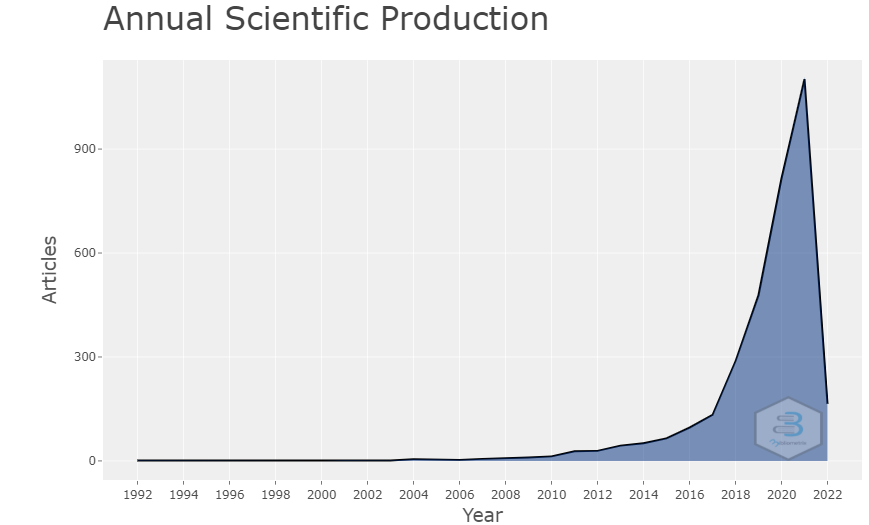
\includegraphics[width=1\textwidth]{experiments/StrawHat972/PesqBibliogr/IA-DeteccaoMalware/WoS-20220209/Imagens/AIMDAnnualScientificProduction.png}
    \caption{Evolução da produção científica no \dataset\ AIMD@StrawHat972}
    \label{fig:StrawHat972:AnnualSciProduction}
\end{figure}

\subsection{Evolução das Citações}
\label{StrawHat972:EvolCit}

A figura \ref{fig:StrawHat972:CitationPerYear} mostra a evolução média de citações aos 3.355 artigos no \dataset\ AIMD@StrawHat972. É notório ao observar o gráfico que o comportamento do mesmo é um tanto quanto irregular apresentando picos de citações seguidos de quedas muito bruscas. Sendo que os maiores picos foram em 2006 (9,9 citações médias), 2007 (9,4 citações médias), 2010 (7,7 citações médias), 2016 (13 citações médias) e 2018 (7,7 citações médias), o que pode estar atrelado à possibilidade de um dado artigo dentro do \dataset\ ter sido muito citado nesses anos. Mesmo com a falta de estabilidade das citações, é perceptível que desde do ano 2001 todos os anos seguintes tiveram citações acima 2 citações médias por ano.

Ao comparar os gráficos das figuras \ref{fig:StrawHat972:AnnualSciProduction} e \ref{fig:StrawHat972:CitationPerYear} podemos notar que mesmo que o crescimento das produções científicas acerca do tema de interesse tenha se mostrado estável ao longo dos anos, o crescimento das citações médias por ano foram bastante instáveis. Mas mesmo com isso, pode-se notar que em ambos os gráficos percebemos um crescimento em relação à primeira publicação presente no \dataset.

\begin{figure}[H]
    \centering
    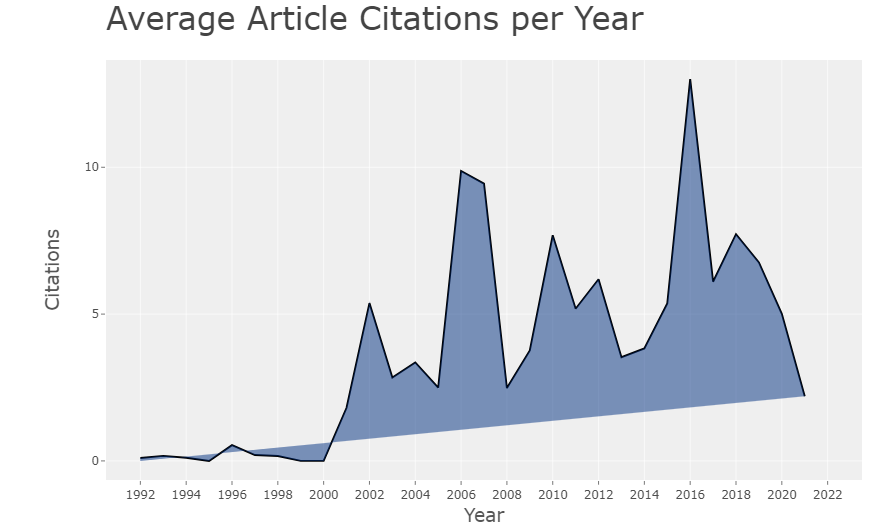
\includegraphics[width=1\textwidth]{experiments/StrawHat972/PesqBibliogr/IA-DeteccaoMalware/WoS-20220209/Imagens/AIMDAverageCitationsPerYear.png}
    \caption{Evolução das citações ao \dataset\ AIMD@StrawHat972}
    \label{fig:StrawHat972:CitationPerYear}
\end{figure}

Com o que foi visto nas seções \ref{StrawHat972:EvolProd} e \ref{StrawHat972:EvolCit}, conseguimos contemplar como se deu a evolução das pesquisas sobre detecção de \textit{Malware} com auxílio de Inteligência Artificial respondendo assim a segunda questão presente na seção \ref{StrawHat972:PlanEst}.

\subsection{\textit{Three-Field Plots (Sankey diagram)}}

O termo \textit{Three-Field Plots} refere-se a uma plotagem de "Três Campos" que demonstra a correlação entre três conjuntos de atributos distintos do \dataset. Na figura, \ref{fig:StrawHat972:ThreeFieldPlot} mostra a plotagem "Três Campos" do \dataset\ AIMD em análise, relacionando, no meio, os 20 Autores mais importantes, na esquerda, as 20 Citações mais frequentes e, na direita, as 20 Palavras-Chave mais utilizadas pelos autores.

Analisando a figura \ref{fig:StrawHat972:ThreeFieldPlot} podemos verificar que a grande maioria dos 20 autores mais relevantes são provavelmente de origem asiática, levando em consideração os sobrenomes. Isso se deve principalmente pelo grande destaque da comunidade chinesa no campo da Inteligência Artificial, o que se deve à ascensão da China como uma potencial tecnológica.

Quanto aos termos mais frequentemente usados como palavras-chave pelos autores, podemos ver que todas as 20 palavras-chave se adéquam a \query\ de busca que foi ilustrada na listagem \ref{StrawHat972:QueryAIMD}. Termos como \textit{Machine Learning}, \textit{Deep Learning}, \textit{Feature Extraction} ou \textit{Training} são termos relacionados à aplicação de técnicas da Inteligência Artificial, visto que nos interessa descobrir como aplicar tais técnicas para a detecção de \textit{Malware}. Agora, em relação às palavras-chave como \textit{Malware}, \textit{Malware Detection}, \textit{Security} ou \textit{Internet of Things}, todos esse são termos relacionados com cibersegurança, que é o cerne do nosso estudo, visto que o objetivo desse tema é descobrir como fazer uma detecção precisa de \textit{softwares} maliciosos.

Por fim, com relação aos artigos mais citados, é perceptível que esses artigos se distribuem em um intervalo de tempo que vai desde 1995 até 2016 destacando que a maioria desses artigos são de 2010 para frente, mostrando que nos últimos 6 não houve nenhuma mudança notória no paradigma do tema de interesse.

\begin{figure}[H]
    \centering
    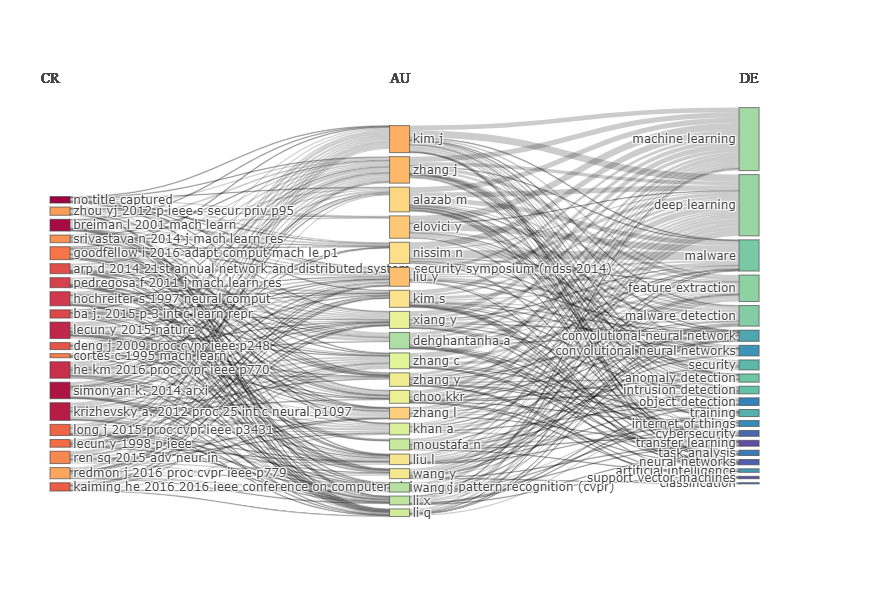
\includegraphics[width=1\textwidth]{experiments/StrawHat972/PesqBibliogr/IA-DeteccaoMalware/WoS-20220209/Imagens/AIMDThreeFieldPlot.png}
    \caption{Plotagem "Três Campos" do \dataset\ AIMD@StrawHat972: 20 Autores, Citações e Palavras-Chave mais relevantes}
    \label{fig:StrawHat972:ThreeFieldPlot}
\end{figure}

\section{Análise da estrutura intelectual}

A fim de entender como é a estrutura intelectual do \dataset\ em questão, isto é, como que os autores ou artigos citam trabalhos de outras pessoas, é necessário levar em consideração a \textbf{Rede de Co-citação} do \dataset\ AIMD@StrawHat972 presente na figura \ref{fig:StrawHat972:CocitationNet}.

\begin{figure}[H]
    \centering
    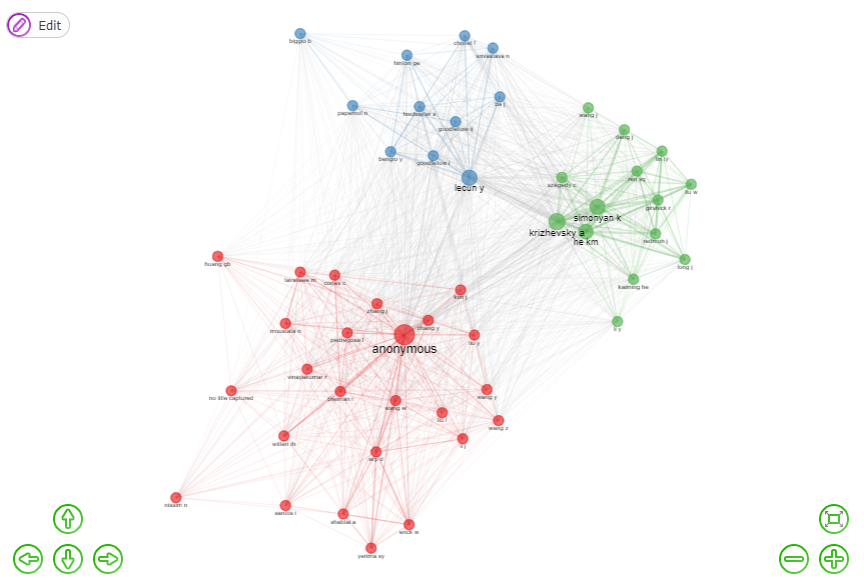
\includegraphics[width=0.8\textwidth]{experiments/StrawHat972/PesqBibliogr/IA-DeteccaoMalware/WoS-20220209/Imagens/AIMDCocitationNetwork.png}
    \caption{Rede de Co-citação do \dataset\ AIMD@StrawHat972}
    \label{fig:StrawHat972:CocitationNet}
\end{figure}

É fácil notar que a Rede de Co-citação se divide em 3 aglomerados principais. O \textit{cluster} azul é o menor dos três e tem \textit{Lecun} como principal autor citado. No caso do conglomerado verde, que é ligeiramente maior que o azul, podemos perceber que os autores que são foco das citações nesse grupo são os autores \textit{Simonyan} e \textit{Krizhevsky}. Por fim, para o aglomerado vermelho se encontra uma situação bastante peculiar.

Observando o grafo, é evidente que o autor \textit{Anonymous}, além de ser o foco de citação do \textit{cluster} vermelho, é também o autor mais citado em toda a rede. Um fato curioso é que \textit{Anonymous} não é exatamente o nome de uma pessoa, mas sim a expressão que substitui o nome do autor quando esse é anônimo. Com isso, não dá para saber se esse \textit{Anonymous} está referindo-se a um autor anônimo em particular ou um conjunto de autores anônimos, o que pode explicar o fato dele ser o mais citado em toda a rede.

\section{Análise da estrutura conceitual}

Nessa seção será feita análise da estrutura conceitual do \dataset\ em estudo, para compreender quais são os conceitos mais relevantes relacionados ao tema de interesse, visto que esse é um dos objetivos desse projeto. Para tal, vamos observar e analisar a \textbf{Rede de Co-ocorrência} do \dataset\ AIMD@StrawHat972.

\begin{figure}[H]
    \centering
    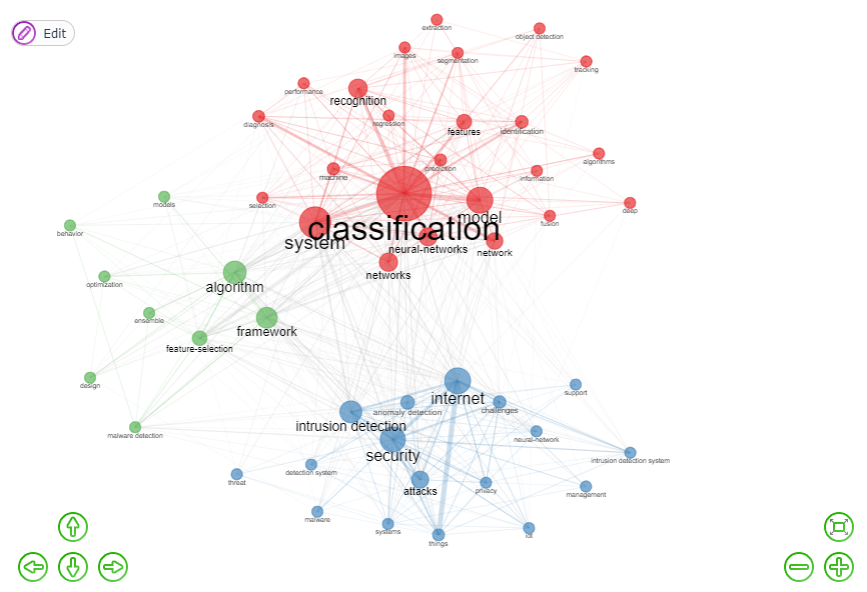
\includegraphics[width=1\textwidth]{experiments/StrawHat972/PesqBibliogr/IA-DeteccaoMalware/WoS-20220209/Imagens/AIMDCooccurrenceNetwork.png}
    \caption{Rede de Co-ocorrência do \dataset\ AIMD@StrawHat972}
    \label{fig:StrawHat972:CooccurenceNet}
\end{figure}

Pelo grafo, é possível verificar que os termos do \dataset\ AIMD podem ser divididos em três setores. No setor vermelho se encontram os termos relacionados com Inteligência Artificial, com destaque para \textit{Classification} que é o conceito que predomina nesse agrupamento. Os conceitos presentes no grupo vermelho estão todos de acordo com o escopo da temática, visto que são termos relacionados com detecção ou reconhecimento de padrões, que é o principal enfoque do tema, ou termos relacionados com aplicações de Inteligência Artificial, que também é interessante para essa análise visto que uma das finalidades para esse estudo é entender como aplicar Inteligência Artificial para detectar \textit{malwares}.

O grupo em azul se caracteriza por conter os termos relacionados com cibersegurança, com destaque para \textit{Security} e \textit{Internet} que são os termos predominantes. Assim como foi no caso do setor vermelho, os termos contidos nesse agrupamento também são dentro do escopo do tema, uma vez que são termos ou relacionados com segurança ou relacionados com a internet cujo acesso se tornou comum o que por consequência facilitou a disseminação de \textit{malwares}.

Por fim, os termos do setor verde de certa forma também estão de acordo com o tema de interesse. Como podemos ver pelo grafo, os conceitos \textit{Algorithm} e \textit{Framework} prevalecem nesse agrupamento. A princípio esses termos parecem não ter tanto a ver assim com o objeto de estudo, entretanto é preciso ter em mente que o tema de interesse trata-se de como utilizar a Inteligência Artificial para detectar \textit{malwares} de forma mais precisa, então implicitamente o objetivo desse tema é nada mais do que desenvolver uma ferramenta tecnológica capaz de de atender a premissa. Levando isso em consideração, é fácil agora perceber que esses termos no agrupamento verde também estão dentro do escopo temático.

Para contemplar totalmente a primeira questão que norteia esse estudo, além da análise da Rede de Co-ocorrência, é fundamental uma inspeção em cima da \textbf{Análise Fatorial} do \dataset\ AIMD@StrawHat972 a fim de compreender corretamente como se dá a estrutura conceitual do mesmo.

\begin{figure}[H]
    \centering
    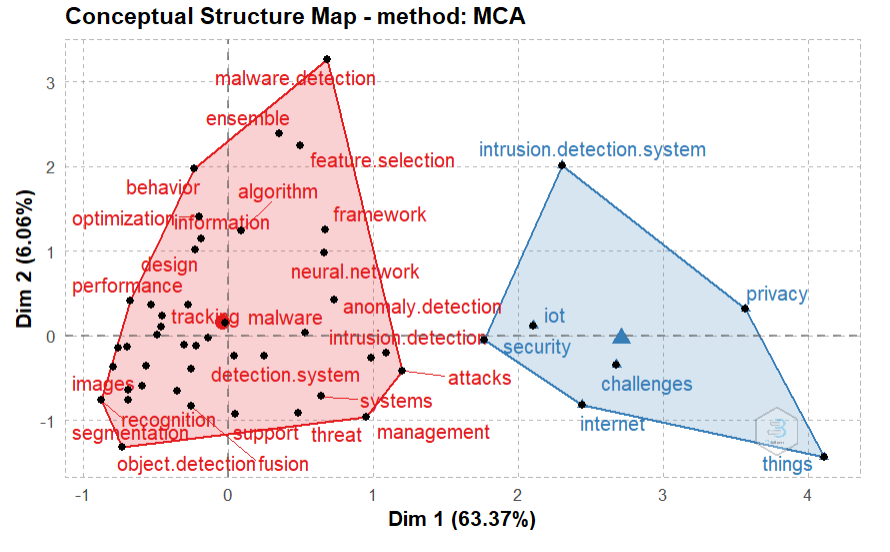
\includegraphics[width=0.8\textwidth]{experiments/StrawHat972/PesqBibliogr/IA-DeteccaoMalware/WoS-20220209/Imagens/AIMDFactorialAnalysis.png}
    \caption{Estrutura Conceitual do \dataset\ AIMD@StrawHat972}
    \label{fig:StrawHat972:FactorialAnalysis}
\end{figure}

Como podemos observar na figura \ref{fig:StrawHat972:FactorialAnalysis}, os conceitos do nosso \dataset\ estão agrupados em dois \textit{clusters} distintos, um em vermelho que abrange grande parte dos conceitos que estão relacionados com detecção, Inteligência Artificial e ameaças de segurança, e um em azul com menos termos e que os conceitos estão associados principalmente à internet, ou seja, estão focados na parte "ciber" da cibersegurança. Vale notar também, que os termos \textit{Algorithm} e \textit{Framework}, e os demais membros que faziam parte do agrupamento verde na Rede de Co-ocorrência da figura \ref{fig:StrawHat972:CooccurenceNet}, estão dentro do \textit{cluster} vermelho, o que de certa corrobora com a argumentação feita anteriormente.

Com isso, fica claro quais os conceitos mais relevantes sobre o tema e como eles estão estruturados o que responde a primeira pergunta presente na seção \ref{StrawHat972:PlanEst}.

\section{Análise da estrutura social}

Por fim, resta responder a última pergunta da seção \ref{StrawHat972:PlanEst}, que se trata de saber como se dá estruturação social dos pesquisadores dentro dessa temática. Para isso, faremos a análise de \textbf{Redes de Colaboração} do \dataset\ AIMD@StrawHat972.

\begin{figure}[H]
    \centering
    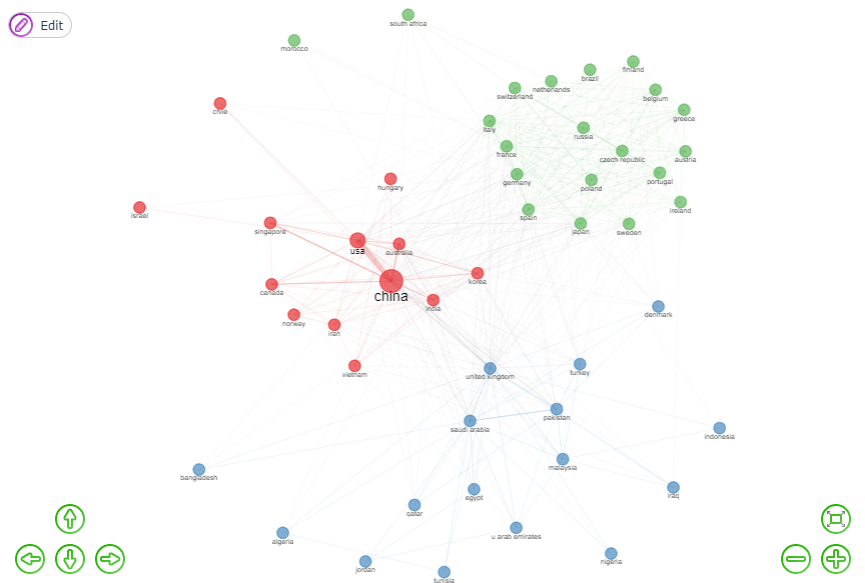
\includegraphics[width=0.8\textwidth]{experiments/StrawHat972/PesqBibliogr/IA-DeteccaoMalware/WoS-20220209/Imagens/AIMDCollaborationNetworkCountries.png}
    \caption{Rede de Colaboração dos países no \dataset\ AIMD@StrawHat972}
    \label{fig:StrawHat972:CollabNetC}
\end{figure}

Na figura \ref{fig:StrawHat972:CollabNetC} é ilustrada a Rede de Colaboração entre os Países. Como pode-se notar, os países se dividem em três grupos. O grupo verde é o mais unido e consiste na sua maioria por países europeus, com algumas exceções como é o caso do Brasil, Japão, África do Sul e Marrocos, dessa certa pode ser visto como um núcleo europeu. O grupo azul é mais disperso e os países em sua maioria são de origem asiática, mas também ocorre casos de países europeus e africanos. Por fim, fica evidente que no grupo vermelho há um núcleo sino-americano, em que a China e os Estados Unidos são os países que mais colaboram nesse \textit{cluster}, além disso o agrupamento vermelho tem a maioria dos países de origem asiática.

Observando o grafo, é fácil perceber que os países que mais colaboram para as pesquisas sobre o uso de Inteligência Artificial para detecção de \textit{softwares} maliciosos são, em primeiro lugar, a China e, em segundo lugar, os Estados Unidos. Além disso, podemos notar que a Rede de Colaboração tem em sua maioria países de origem euro-asiática.

\begin{figure}[H]
    \centering
    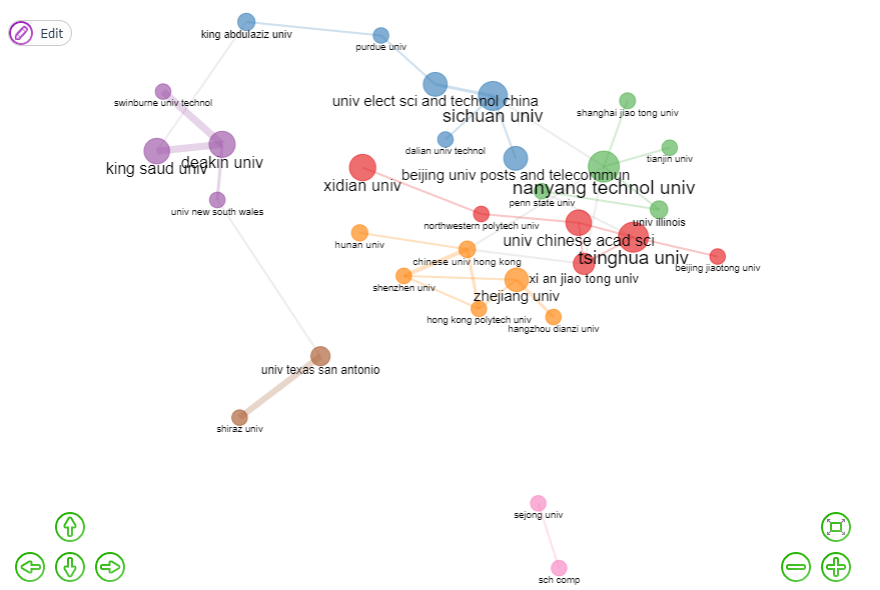
\includegraphics[width=1\textwidth]{experiments/StrawHat972/PesqBibliogr/IA-DeteccaoMalware/WoS-20220209/Imagens/AIMDCollaborationNetworkIntitutions.png}
    \caption{Rede de Colaboração das instituições no \dataset\ AIMD@StrawHat972}
    \label{fig:StrawHat972:CollabNetI}
\end{figure}

Na figura \ref{fig:StrawHat972:CollabNetI} temos a Rede de Colaboração das instituições. Olhando para o grafo, é notório perceber que existem sete diferentes aglomerados. Em geral, os aglomerados são de universidades chinesas, mas há também aglomerados de universidades americanas, como é caso do aglomerado marrom que temos a universidade de \textit{Texas}. Vale notar também, que temos um aglomerado bastante afastado dos outros, que é o grupo do cor rosa. No caso, tratam-se de instituições de origem sul-coreana, como é caso da universidade de \textit{Sejong}.

Olhando como se deu a disposição dessa Rede de Colaboração das instituições, é perceptível novamente o predomínio da China nesse campo de pesquisa.

\begin{figure}[H]
    \centering
    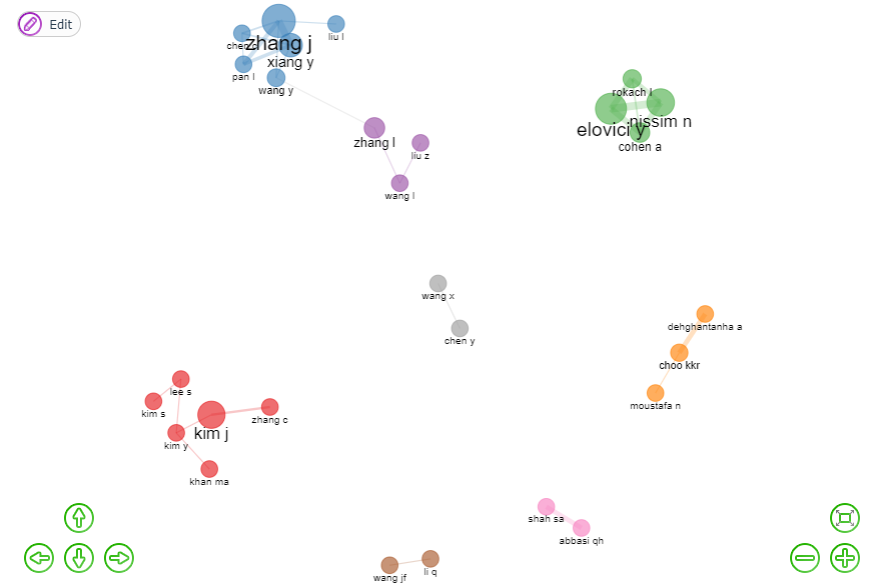
\includegraphics[width=1\textwidth]{experiments/StrawHat972/PesqBibliogr/IA-DeteccaoMalware/WoS-20220209/Imagens/AIMDCollaborationNetworkAuthors.png}
    \caption{Rede de Colaboração dos autores no \dataset\ AIMD@StrawHat972}
    \label{fig:StrawHat972:CollabNetA}
\end{figure}

Por último, na figura \ref{fig:StrawHat972:CollabNetA} temos a Rede de Colaboração dos autores do \dataset. Como podemos verificar temos 8 \textit{clusters} bem distintos nessa rede, o que pode estar relacionado a forma que a comunidade chinesa se organiza, sendo mais questão cultural essa disposição gráfica. Os autores com mais destaque em colaboração são os autores \textit{Zhang} do grupo azul, \textit{Elovici} do grupo verde e \textit{Kim} do grupo vermelho. Percebemos novamente que o maior \textit{cluster} é composto principalmente por pesquisadores chineses, como evidenciado na análise das demais redes.

Por fim, com o que foi visto nas análises das Redes de Colaboração temos agora um panorama de como é a estrutura social do tema de interesse, o que responde, assim, a nossa última pergunta presente na seção \ref{StrawHat972:PlanEst}, contemplando de todos os objetivos desse projeto.

\section{Conclusão}

Por meio dessa análise bibliográfica, fomos capazes de compreender quais eram os conceitos mais relevantes sobre o uso de Inteligência Artificial para a detecção de \textit{malwares}. Além disso, também contemplamos como se deu a evolução das pesquisas referentes a esse tema ao longo dos anos e percebemos que esse teve um crescimento de caráter exponencial, apresentando um grande crescimento nos últimos. Por fim, também conseguimos entender como é a estrutura das comunidades que trabalham em cima dessa temática, e compreendemos que em sua maioria temos uma predominância por parte de pesquisadores chineses.

No que diz respeito ao próprio estudo, foi empregado para a realização do mesmo muito mais esforço e tempo que fora planejado anteriormente. Entretanto, essa maior dedicação resultou em uma boa experiência na utilização da técnica da análise bibliográfica que se demonstrou uma técnica muito importante para se compreender qual o contexto acadêmico geral de um tema de interesse. Em razão disso, com certeza tal técnica será usada para trabalhos futuros para enriquecer o estudo.